\documentclass{article}
\usepackage[utf8]{inputenc}

\usepackage[T1]{fontenc}
\usepackage{amssymb}
\usepackage[swedish]{babel}
\usepackage{amsmath}
\usepackage{lmodern}
\usepackage{units}
\usepackage{icomma}
\usepackage{color}
\usepackage{graphicx}
\usepackage{bbm}
\usepackage{hyperref}
\usepackage{pdfpages}
\usepackage[makeroom]{cancel}

\setlength{\parindent}{0em}
\setlength{\parskip}{0.5em}

\begin{document}

\begin{titlepage} \newcommand{\HRule}{\rule{\linewidth}{0.3mm}}
\center
\textsc{\Large Chalmers tekniska högskola}\\[0.05cm] % Name of your university/college \textsc{\normalsize Teknisk Matematik}\\[0.2cm]
%\normalsize \\ % Major heading such as course name
\normalsize \today

\HRule \\[0.08cm]
{ \large Planeringsrapport \\ \normalsize{-- Programmering som undervisningsverktyg för signaler och system}}\\[0.08cm] %Signalteori är för stort?
\HRule \\[0.3cm]

\vfill

\begin{flushleft} \small
    \emph{Author: \\
    \quad Filip Lindahl\\
    \quad Cecilia Rosvall\\
    \quad Peter Ngo\\
    \quad Jacob Jonsson\\
    \quad Joakim Olsson\\}
\end{flushleft}
\end{titlepage}
\newpage
%\tableofcontents
%\newpage

\section{Bakgrund}
På Chalmers tekniska högskola har det funnits en lång trend där
studenterna på utbildningen för Datateknik har haft svårigheter med
kurserna ``Transformer, Signaler och System'' (TSS) och
“Reglerteknik”. Dessa svårigheter tror examinatorerna i kurserna beror
till stor del på att studenterna inte är tillräckligt bekväma i det
matematiska språket. Studenterna på Datateknik har inte tillräcklig
vana att tolka innebörden av de matematiska beskrivningarna.

Detta syns bland annat i statistiken för hur många
datastudenter som klarar kurserna, under perioden från
2010 till 2016 blev i genomsnitt 49\% av alla som skrev
tentamen underkända i TSS och under samma period blev
47\% underkända i Reglerteknik.
%TODO: Ange andelen som klarar istället (för att matcha början på meningen och för att passa ihop med begrepped "genomströmning")
%TODO: Kolla vad genomsnittlig genomströmning är för kurserna i D3 eller hela kandidatdelen av D för att ge läsaren en chans att "kalibrera".
Det finns även ett mörkertal i dessa siffror eftersom inte alla studenter skriver tentan.
%TODO: Det vore bra att ange något slags mått på detta "mörkertal". Kanske genom att ange andelen som klarar kursen jmf. med antalet studenter registrerade den terminen?

För att minska svårigheterna som studenterna har för dessa kurser
påbörjades ett pedagogiskt projekt (DSLsOfMath) som hittills
resulterat i kursen “Matematikens domänspecifika språk”, där man
använder funktionell programmering för att beskriva matematiska problem.
Resonemanget bakom detta var att funktionell programmering är ett
verktyg som datastudenterna har erfarenhet av och som använder en
notation med fokus på tydlighet som lämpar sig relativt väl för
att lära ut matematiska begrepp.

Vårt projekt uppstod som en avgrening av DSLsOfMath-projektet med
fokus mer på signal- och systemteoretiska färdigheter snarare än
en allmän matematisk grund.

\section{Syfte}
Syftet med projektet är att underlätta för studenter inom datateknik
att ta till sig signal- och systemteoretiska ämnen genom att utnyttja
deras kunskaper inom programmering och även göra det möjligt att
betrakta ämnet ur en programmerares perspektiv.
Med detta hoppas man göra gapet mellan datateknik och
signalteori mindre och minska problemen som nämns i
bakgrundsavsnittet.

Projektet är tänkt att resultera i en handledningsguide, en så kallad
tutorial, som kan fungera som ett komplement till de kurser som ges
inom signalteori på den datatekniska grundutbildningen. Denna guide ska innehålla förklaringar och programmeringsövningar som är anpassade för studenter på den datatekniska utbildningen.
%Bra!
\section{Problemanalys}
Uppgiften i detta projekt är att utarbeta en tutorial som
komplement till kurserna “Reglerteknik” och “Transformer, signaler och
system”.

För att kunna utveckla denna ``produkt'' kommer först omfattande
%TODO: det är lite oklart att i första meningen skriva "uppgift" och
%sedan plötsligt "produkt". Om ni vill fortsätta använda "produkt"
%behöver denna övergång göras tydlig.
%ASE: varför inte fortsätta säga tutorial istället för produkt?
förstudier behöva bedrivas innan vi utvecklar vår produkt och denna
produkt kommer sedan behöva testas.
%TODO: Undvik upprepning: här 3*produkt i samma mening


\subsection{Förstudier}
För att komma till rätta med datastudenternas största svårigheterna
med förståelsen inom ämnena behöver vi först undersöka var dessa
svårigheter ligger mer i detalj.

%TODO: skriv mer direkt: "kommer vi även behöva bedriva en hel del" är onödigt krångligt skrivet
Dessutom kommer vi även behöva bedriva en hel del efterforskningar
och litteraturstudier inom såväl pedagogik som de signalteoretiska
ämnen vi beskriver för att kunna skriva en produkt med korrekt och
tydligt innehåll.
%TODO: Allmänt sätt vore det bra att minska antalet "behöva" i texten. Strikt sett är det inte en plan att säga att något behövs. Många saker "behövs" men ni väljer att verkligen göra vissa saker. Fokusera på vad ni ska göra, inte på vad som behöver göras.

\subsection{Produkten}
Efter förstudierna kommer en tutorial utvecklas.
%
Innehållet i denna kommer bestå av förklarande teori,
exempel inom såväl teori som programmering, samt övningar
med tillhörande lösningar.

\subsection{Testa produkten}
Produkten kommer sedan behöva testas på den aktuella målgruppen för
möjligheten att uppdatera och förbättra den slutgiltiga produkten.

\section{Avgränsning}
%TODO: Var tydlig med om ni anser att "handledningsguide" är samma som "tutorial". (Alternativ översättning är "lathund", "vägledning", "studiehäfte", ...)
I detta projekt skrivs en handledningsguide vars avsikt är att
förtydliga de delar studenter inom datateknik finner svårt i kurserna
“Transform, Signal och System” och “Reglerteknik”.
%
Detta innebär att vi endast fokuserar på svårigheter inom dessa kurser
och inte ett alternativt läromaterial som täcker hela själva ämnet.
%
Det vill säga, produkten kommer inte bli ett underlag för motsvarande
kurs DAT325 utan ett komplement till kurserna SSY080 och ERE103.
%TODO: tydliggör kopplingen mellan koderna och kurserna. Jag föreslår att etablera förkortningar (TSS, Regler) och sedan använda dem istället för koderna. Sedan bör det finnas en sektion med referenser där koderna och länkar till kursplaner kan tas med.

\section{Metod}
\subsection{Förstudier}
För att samla in information om vilka moment i kurserna
TSS och Reglerteknik som datastudenter har svårast för har
vi intervjuat examinatorerna om de övergripande
svårigheterna inom båda kurserna.
%Bra!
Vi kommer under projektets gång ha fler intervjuer med
examinatorerna där det läggs mer fokus på detaljer.
Vi planerar också att fråga studenter som har läst
kurserna vad de tyckte var svårast.

För att kunna skriva en lättläst och begriplig tutorial
kommer vi studera litteratur inom pedagogik samt
alternativa inlärningsformer som exempelvis boken och
hemsidan “Learn you a Haskell for great good”.

\subsection{Produkten}
Rent strukturellt planerar vi att dela upp ämnet i
sex delavsnitt som kommer att innehålla informativ text som
förklarar delavsnittet och runt 15 -- 20 uppgifter vardera.
I uppgifterna får studenterna lära sig om signaler och
system genom att implementera de inblandade typerna
och relationerna som domänspecifika språk i Haskell.

\subsection{Testa Produkten}
För att testa svårighetsgraden på vår produkt kommer vi dels att testa
gruppens uppgifter internt och förhoppningsvis hitta utomstående
studenter som är villiga att testa produkten. Från dessa tester kan vi använda feedbacken för att vidareutveckla och förfina slutprodukten.

\section{Tidsplan}
\subsection{Milstolpar och delmål}
\begin{itemize}
\item 2016-02-10 - Planeringsrapport och grov planering klar
\item 2016-02-11 - Fackspråkshandledningstillfälle 1
\item 2016-02-12 - Planeringsrapport inlämning
\item 2016-02-24 - Intervjuer, grundläggande efterforskningar om TSS och reglerkurserna klara
\item 2016-02-24 - Litteraturstudier inom pedagogik klara
\item 2016-03-01 - Utkast för grov tutorial klar (uppgifter ej klara)
\item 2016-03-01 - Få klart ett litet avsnitt för halvtidsredovisningen, med förslag på uppgifter och text
\item 2016-03-01 - Halvtidsredovisning
\item 2016-03-15 - Uppgifter och utkast till text för två av sex delavsnitt i tutorial klara
\item 2016-03-22 - Första utkast till rapporten klart
\item 2016-03-22 - Fackspråkshandledningstillfälle 2
\item 2016-03-28 - Bearbetning av feedback från fackspråk
\item 2016-03-28 - Påsk
\item 2016-04-11 - Uppgifter och utkast till text för fyra av sex delavsnitt i tutorial klara
\item 2016-04-25 - Uppgifter och utkast till alla delavsnitt i tutorial klara
\item 2016-04-27 - Eventuell engelsk (forskningsinriktad) uppsats klar
\item 2016-04-28 - Andra utkast till rapporten klart
\item 2016-05-04 - Tutorial klar och testad
\item 2016-05-11 - Rapporten klar
\item 2016-05-13 - Fackspråkshandledningstillfälle 3
\item 2016-05-16 - Rapportinlämning
\item 2016-05-17 - Utställning
\item 2016-05-26 - Deadline för opposition
\item 2016-05-26/27 - Slutredovisning
\item 2016-06-01 - Sista inlämningen
\end{itemize}

\newpage
\subsection{Gantt schema}
\begin{figure}
    \centering
    %TODO: Gannt stavas Gantt.
    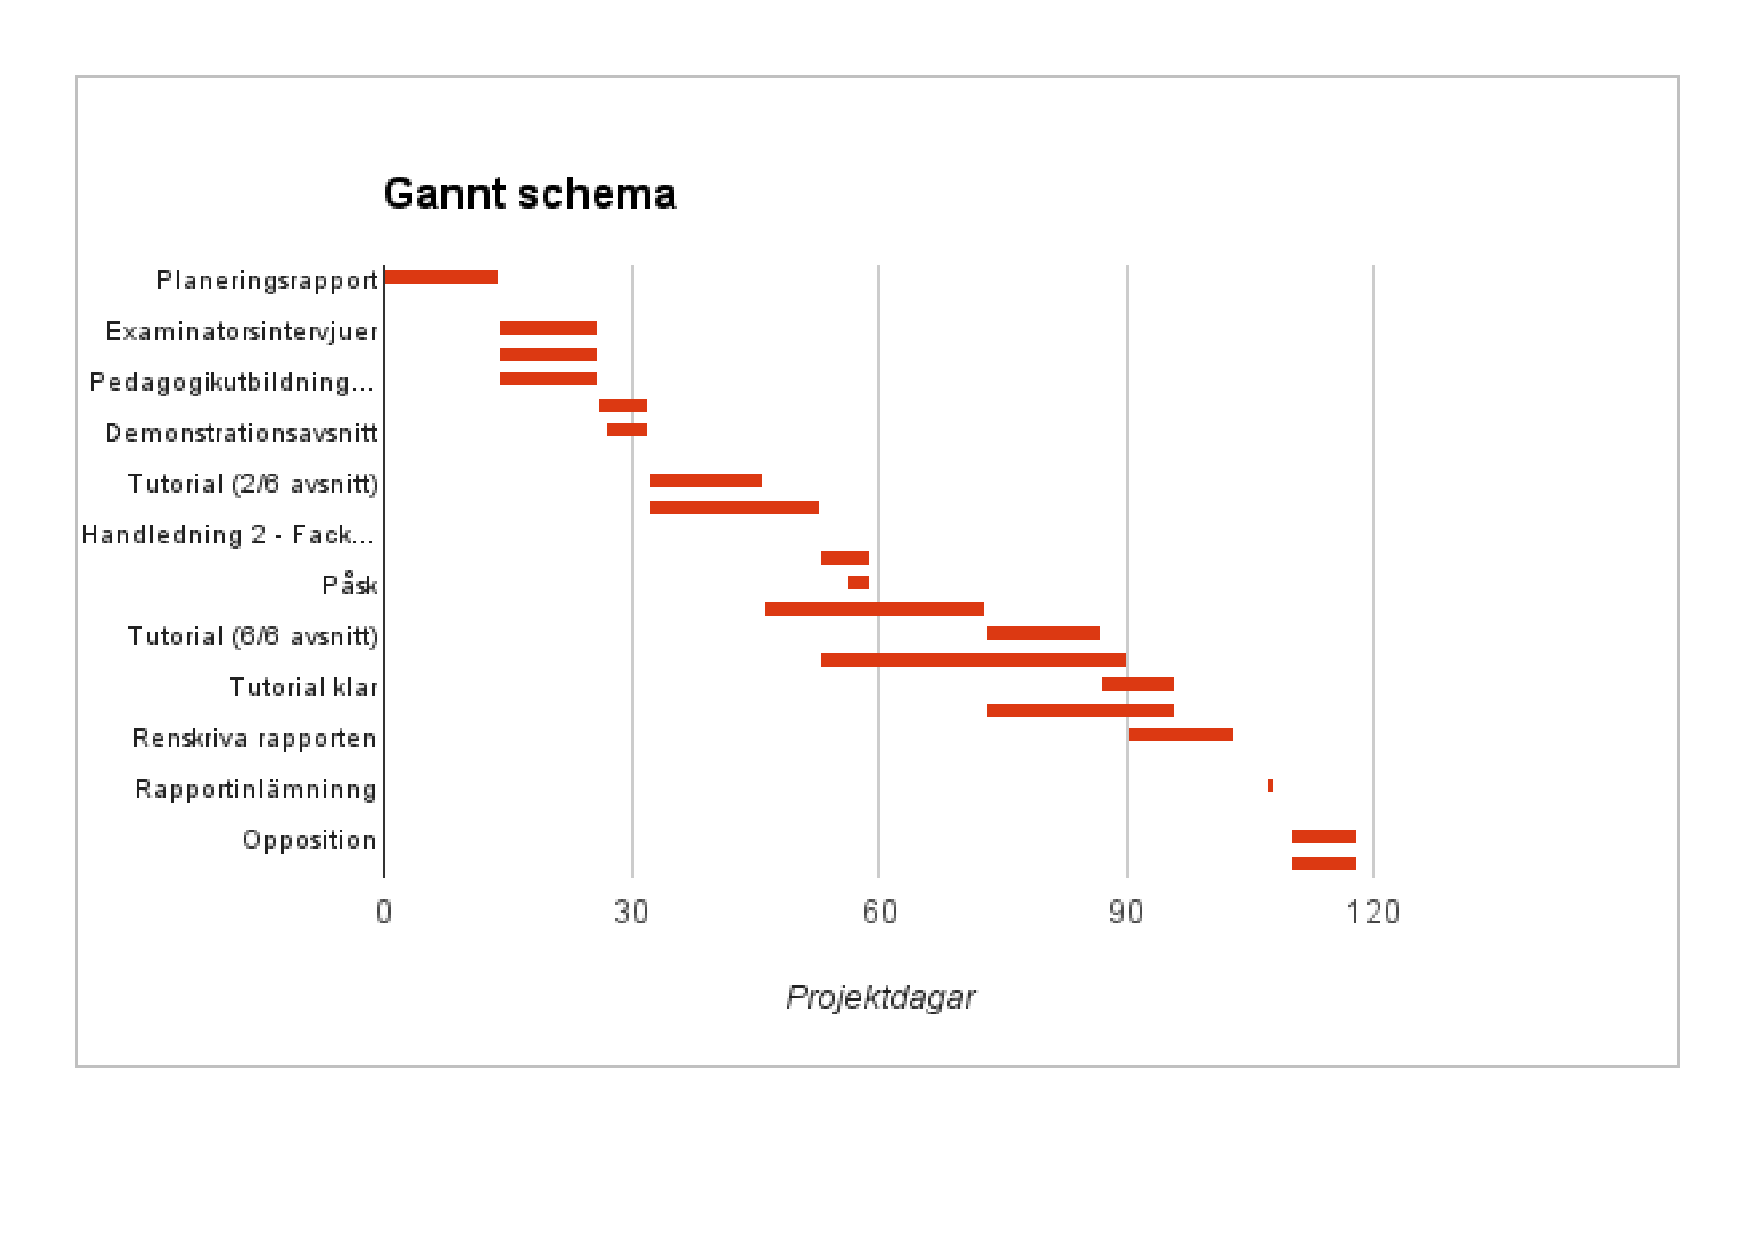
\includepdf[width=0.8\paperwidth]{Gannt}
\end{figure}
\end{document}
